\documentclass[tikz,border=10pt]{standalone}
\begin{document}
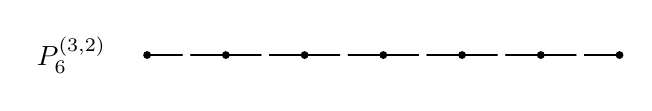
\begin{tikzpicture}[scale=2]
    % Define the points along the path
    \foreach \x in {0, 0.5, 1, 1.5, 2, 2.5, 3} {
        \node[circle, fill=black, inner sep=1pt] at (\x,0) {};
    }
    
    % Draw the path connecting the points
    \draw[thick, black] (0,0) -- (0.5,0) -- (1,0) -- (1.5,0) -- (2,0) -- (2.5,0) -- (3,0);
    
    % Add additional points to emphasize the path
    \node[circle, fill=white, inner sep=1pt] at (0.25,0) {};
    \node[circle, fill=white, inner sep=1pt] at (0.75,0) {};
    \node[circle, fill=white, inner sep=1pt] at (1.25,0) {};
    \node[circle, fill=white, inner sep=1pt] at (1.75,0) {};
    \node[circle, fill=white, inner sep=1pt] at (2.25,0) {};
    \node[circle, fill=white, inner sep=1pt] at (2.75,0) {};
    
    % Add labels for clarity
    \node[left] at (-0.2,0) {$P_6^{(3,2)}$};
\end{tikzpicture}
\end{document}